
\subsection{Case 2: \scipion at the Swedish National Cryo-EM Facility}

The Swedish National Cryo-EM Facility %%offers access to state-of-the-art equipment and expertise in single particle cryo-EM and cryo electron tomography (cryo-ET). The Facility 
has two nodes: at \scilifelab in Stockholm and at Ume\aa\ University. \scilifelab in Stockholm offers single-particle service with a 
Talos Arctica for sample optimisation and a Titan Krios for high-resolution data collection. The Ume\aa\ node offers cryo-ET with a Titan Krios and a Scios DualBeam SEM.
%The facilities can be accessed by Swedish researchers through 
%a peer-reviewed process. Applications can be submitted through an application portal (\url{https://cryoem.scilifelab.se/}). % and will be evaluated once every three months based on their scientific merit and technical feasibility by a national Project Evaluation Committee. %On the other side, some time of the facility is reserved for internal research groups at Stockholm University. 
Internally, an online booking system called \emph{Booked Scheduler} centralizes the reservations of the microscopes and other instruments. 

At the beginning of 2016, the Cryo-EM facility at \scilifelab became one of the early adopters of \scipion streaming processing. Although the microscope operators were using home-made scripts to perform motion correction (with motioncor2) and CTF estimation (with Gctf), they recognized the importance of a more general
framework. In particular, they were interested in the possibility of modifying easily the processing workflow as well as provide users and staff with  graphical tools for data analysis and quick feedback regarding the data collection.
Although initially the same setup script used at
CNB was adopted, a new one was developed to fully satisfy the facility
requirements. In the following sections we will briefly describe the computational infrastructure at the \scilifelab node and the implementation of a Session Wizard to automate the initial setup while fetching information from other sources external to \scipion. %(In this contest wizard refers to a helper script which guide users through a certain process.)
%[** thalos falcon III, titan k2 and falcon III]

\subsubsection{Network Setup and IT Infrastructure}
A storage and pre-processing server (the staging
server) constitutes the core of the SciLifeLab computational infrastructure.
 This machine has roughly 200 TB of storage (4 ZFS RAIDZ2 pools with 11 HDDs each), 2 NVIDIA GeForce GTX 1070 GPUs, 2 Intel Xeon E5-2630v4 CPUs (10 cores, 2.2 GHz, HT), 384 GB RAM, and a dual-port 10 GbE network card. The storage pool is exported via NFS and Samba. The microscope computers can thus write data directly there and other machines can access it.
 
% The storage pool is exported via NFS and Samba, so the microscope computers can write data there directly and other machines can access it.
%Unfortunately, the K2 [** Jose Miguel, what is K2?, do you have 2 cameras? in the same microscope or in different ones, this is confusing, comment when ] computer writes data to a local SSD RAID while the Falcon-III does it to a dedicated storage server. %, in order to avoid interruption of data collection due to network issues. 

%To avoid interruption of data collection due to network issues each microscope has its own dedicated storage, that in the case of the Titan microscope is double since it may be connected to two different cameras, a K2 and a Falcon III. Hence a script to continuously move the produced data from the adequate storage to the staging server has been created. 

%In this way, after starting the data collection, users launch a script that continuously moves the produced data from the adequate storage to the staging server.

%ata on the staging server, in an organized folder structure, we
%can run pre-processing directly on the server.] If data processing is started soon
%after data collection the incoming data file should be in RAM-cache and  no
%disk access in needed, which is important with performance in mind. 
After processing, users may  copy their data to external USB drives from two workstations in the microscope room that have access to the storage pool via NFS.
There is also a dedicated download server which has access to the NFS export. This download server is accessible from  the Internet and allows downloads via rsync (over SSH) or SFTP. 

All these computers are connected to a 10 GbE network switch. The only machine accessible from the Internet is the data download server, which has a dual-port 10 GbE network adapter (one used for the internal network, one for the external network). %Both the K2 computer and the Falcon-III dedicated storage server had one unused 10GbE interface that could be used to connect them to our private network, without having to interfere with the default setup.

\subsubsection{Additional Software Developments: \emph{Session Wizard}}
In order to interface \scipion with the microscope infrastructure, an upgraded version of the original script developed at CNB was used. Unfortunately, it was difficult to reuse the existing code due to a different folder structure and, more important, a different approach to user and microscope management. To address the new set of requirements, a new wizard has been developed at \scilifelab (see \ffigure{fig:wizard}). %(In this contest wizard refers to a helper script which guide users through a certain process.) %For this new wizard, a basic data model was designed representing the current processing and data organization at \scilifelab. %The model is composed by the following entities:
\begin{figure}
\hspace*{-2cm}                                                           
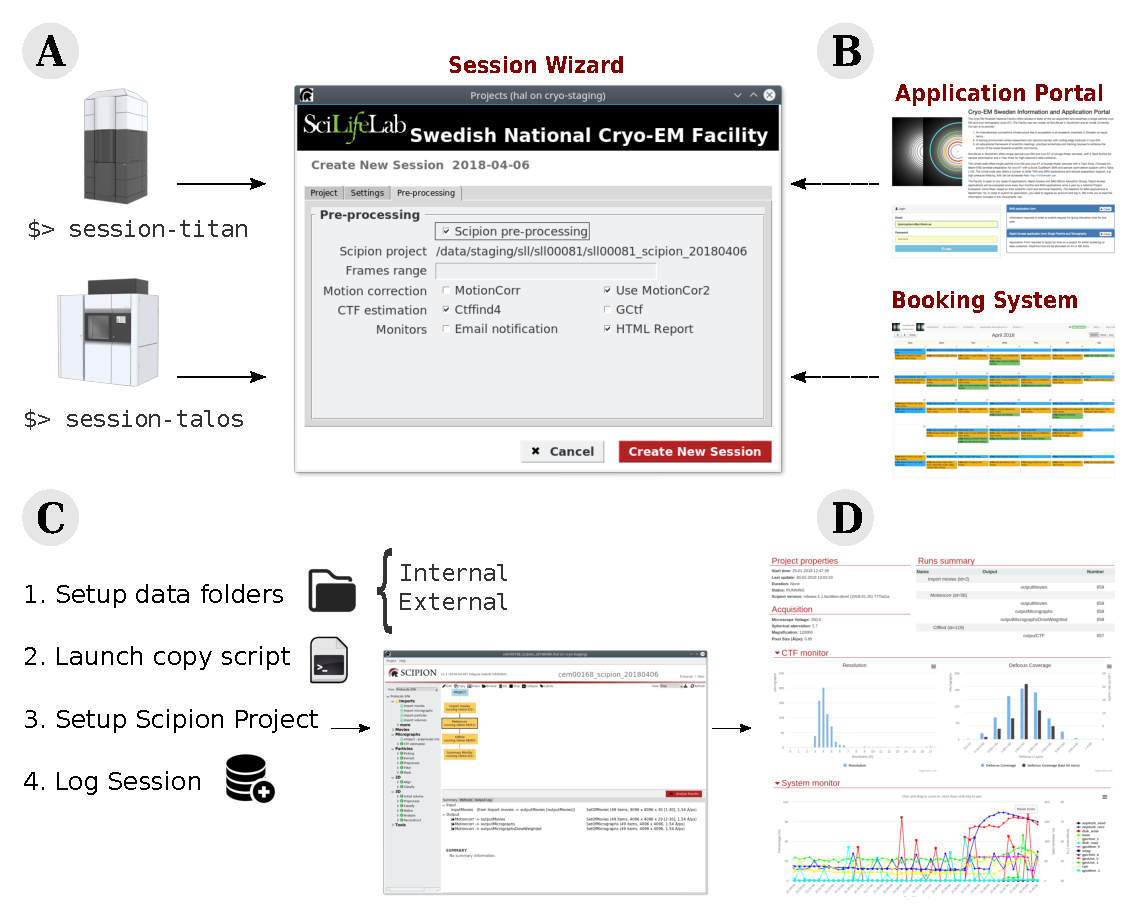
\includegraphics[width=1.25\textwidth]{images/scilifelab.pdf}
  \caption{Overview of the Session Wizard  developed at \scilifelab. A) The user triggers the wizard for any of the current microscopes. B) The wizard retrieves project information from the \textit{Application Portal} and reservation details from the \textit{Booking System}. C) The wizard creates data folders, executes the image copying script, configures the Scipion streaming project and logs the current session into a database. D) The \scipion project is used to generate on the fly web reports and invoice documents later on.}
  \label{fig:wizard}

\end{figure}

%[** quitar modelo de datos]
%\begin{itemize}
%\setlength\itemsep{0em}
% \item \textit{User}: represents all persons that can book microscope time or are registered in the Application Portal 
% related to national projects.
% \item \textit{Reservation}:  is a resource (e.g, Krios, Talos, Vitrobot, etc) booking for a given period of time.
% \item \textit{Order}:  is a given national project with an unique identifier in the Application Portal
% \item \textit{Project}:  can be a either a national project (related to a given Order) or an internal project.
% \item \textit{Session}:  stores information about the usage of the micrograph for a given day.
%\end{itemize}

When a user starts a data collection, the wizard is executed using the command \textit{session-titan} (or \textit{session-talos}). The wizard determines which user has booked the microscope by fetching today's booking information from \emph{Booked Scheduler} through their web API, %From the reservation information the wizard will also detect if it is an internal or a national facility project. 
%In case of the latter, additional information will be retrieved from the Application Portal (such as principal investigator, project code, contact person or invoice address). 
%After gathering all this information the wizard 
stores it, creates the processing environment and launches \scipion. %For example, the movies-import protocol will already point to the location where the files will be written for this session. Moreover, taking into account which microscope-camera is being  used, the files pattern can be inferred. 
The current implementation of the wizard stores each session in a simple database file. This database, together with extra information from the Booking System and an Application Portal, is used to generate invoices and reports for a given period. %The generation of a session report is under development, that will provide a summary and useful information for users to access the acquired data. 
%[** this last sentence is not very informative]

The described session wizard can be found at  
\url{https://github.com/delarosatrevin/scipion-session}. The software can be freely downloaded and customized to meet the specific requirements of client organizations. \emph{Booked Scheduler} is available at (\url{https://www.bookedscheduler.com/})

%existing data model represents the specify usage at the \scilifelab facility and there are not immediate plans to make it more general and easy to reuse. Nonetheless, the model is quite simple and should to be difficult to modify it to fit other requirements. 


